\section{Experimental Results}

\subsection{Joint Action Distributions \& Payoffs}
In the Figure~\ref{fig:mallm_matrix}, we present the empirical frequencies of joint outcomes (CC, CD, DC, DD) of the "prisoner's dilemma" game.

Compared to the baseline scenario without communication (Figure~\ref{fig:baseline_comparison}), we observe a significant increase in the frequency of mutual cooperation (CC), when agents are allowed to communicate.
This suggests that pre-play communication can effectively facilitate coordination and enhance cooperative behavior, even in a setting where the Nash equilibrium favors defection.

We can also analyze the average payoffs for each player under different communication conditions:

\begin{table}[htbp]
    \centering
    \begin{tabular}{c|c|c}
        Strategy  & Player A        & Player B        \\
        \hline
        Cooperate & $2.56 \pm 1.07$ & $2.53 \pm 1.09$ \\
        Defect    & $2.09 \pm 1.79$ & $2.04 \pm 1.76$ \\
    \end{tabular}
    \caption{Average payoffs for each player under different communication conditions.}
    \label{tab:average_payoffs}
\end{table}

To be sure of the correctesness of the generated data

\begin{figure}[htbp]
    \centering
    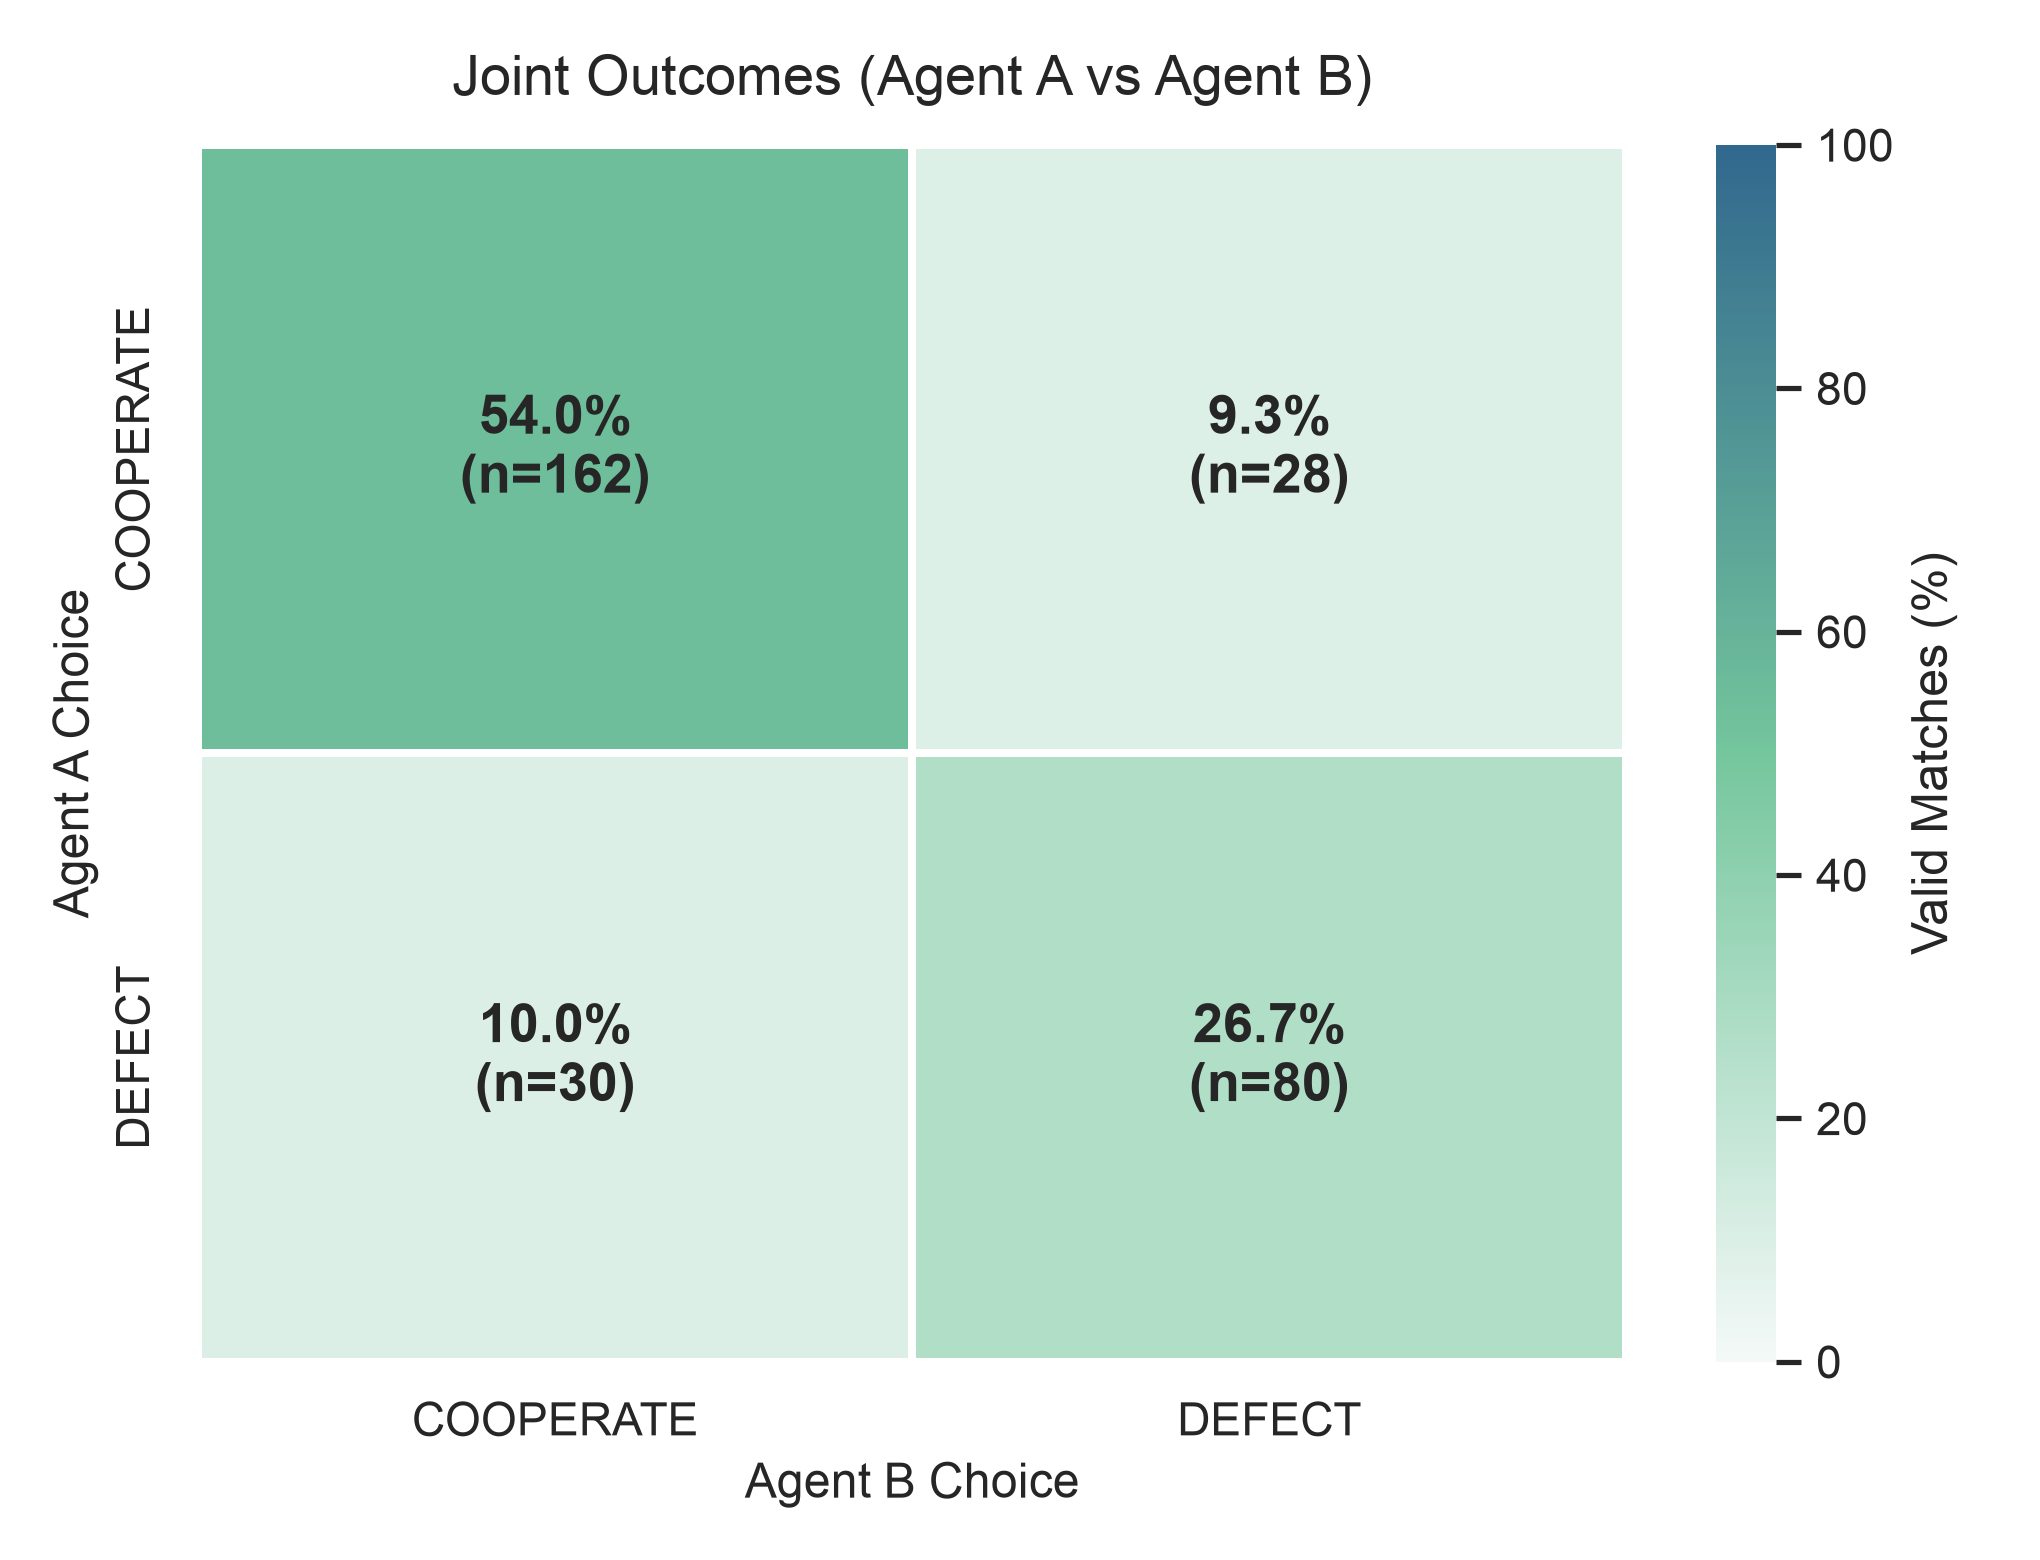
\includegraphics[width=\linewidth]{../..//reports/outcome_matrix_heatmap.png}
    \caption{Matrix of joint action distributions for the prisoner's dilemma game.}
    \label{fig:mallm_matrix}
\end{figure}

\begin{figure}[htbp]
    \centering
    % TODO: change the path of the image
    %\includegraphics[width=\linewidth]{../..//reports/baseline/baseline_comparison.png}
    \caption{Comparison between joint action distributions with and without communication.}
    \label{fig:baseline_comparison}
\end{figure}

\subsection{Alignment, Deception \& Linguistic Patterns}
% TODO: Analyze consistency between diplomatic promises, private [JUDGE] explanations, and actual chosen actions.
% TODO: Discuss verbosity effects (message word count vs probability of cooperation/defection) referencing Figure~\ref{fig:mallm_plot}.

\begin{figure}[htbp]
    \centering
    % TODO: Copy your selected PNG from MALLM intel output into figures/ and uncomment below
    %\includegraphics[width=\linewidth]{reports/your_mallm_plot.png}
    \caption{Empirical relationship between communication patterns and strategic outcomes.}
    \label{fig:mallm_plot}
\end{figure}

